\documentclass[11pt]{article}

\usepackage{hyperref} % Hyperlinks
\usepackage{subfig} % Package f�r mehrere Grafiken nebeneinander
\usepackage{amsmath}
\DeclareMathOperator{\atantwo}{atan2}

%Zeilenabstand
\linespread{1.5}

\usepackage{pdfpages}

%graphics
\usepackage{graphicx}
\usepackage[margin=01in,includefoot]{geometry}
\usepackage{fancyhdr}
\usepackage{float}

% citation
\usepackage{apacite} % APA Citation
\usepackage{natbib} % Additional bibtex commands

\begin{document}
\includepdf[pages=1]{Cover}


\section{Date Cleaning and Preparation}

\subsection{New York Inspection Data}

The main dataset for our project is retrieved from the \href{https://data.ny.gov/Economic-Development/Retail-Food-Store-Inspections-Current-Ratings/d6dy-3h7r}{official site of the State of New York}. It contains a total of 28'300 A to C ratings of food store inspections together with basic information of the stores as well as deficiency descriptions.\\
\\
Our analysis predicts the food store inspection ratings from this dataset only for the City of New York counties New York, Kings, Bronx, Richmond and Queens). We decided to focus merely on city level due to the vast availability of covariate data. In addition, the distribution of classes is highly imbalanced on state level which can be diminished by focusing on city data only (more about this issue in section~\ref{Imbalance Problem}.

\subsection{Chain Information}

We used the owner information from the data to identify if the shop is a chain as well as the number of other stores from our data that are part of the same chain. Presumably, chains have better processes in place to achieve a high hygiene standards.

\subsection{Spatial Data}

Latitude and longitude information is embedded in a larger address string. We create a function to extract the location data in two new columns. A check for \texttt{NA} values reveals that 748 observations have no location information. The exact address, however, is available for all shops. Therefore, we provide the address to the Google Maps API\footnote{In essence, the Google Maps API is a free service offered by Google. It requires only a one-time registration with a valid email address. Afterwards, it generates an API Key that must be included in the R-script  with the command \texttt{register\_google(key = "API KEY")}.} to retrieve the missing latitude and longitude details. A Map of the completed data is illustrated in Figure~\ref{map1} on state and city level.\\
\begin{figure}
\captionof{figure}{Geographic Distribution of the inspected Shops \label{map1}} 
\subfloat[New York State]{%
       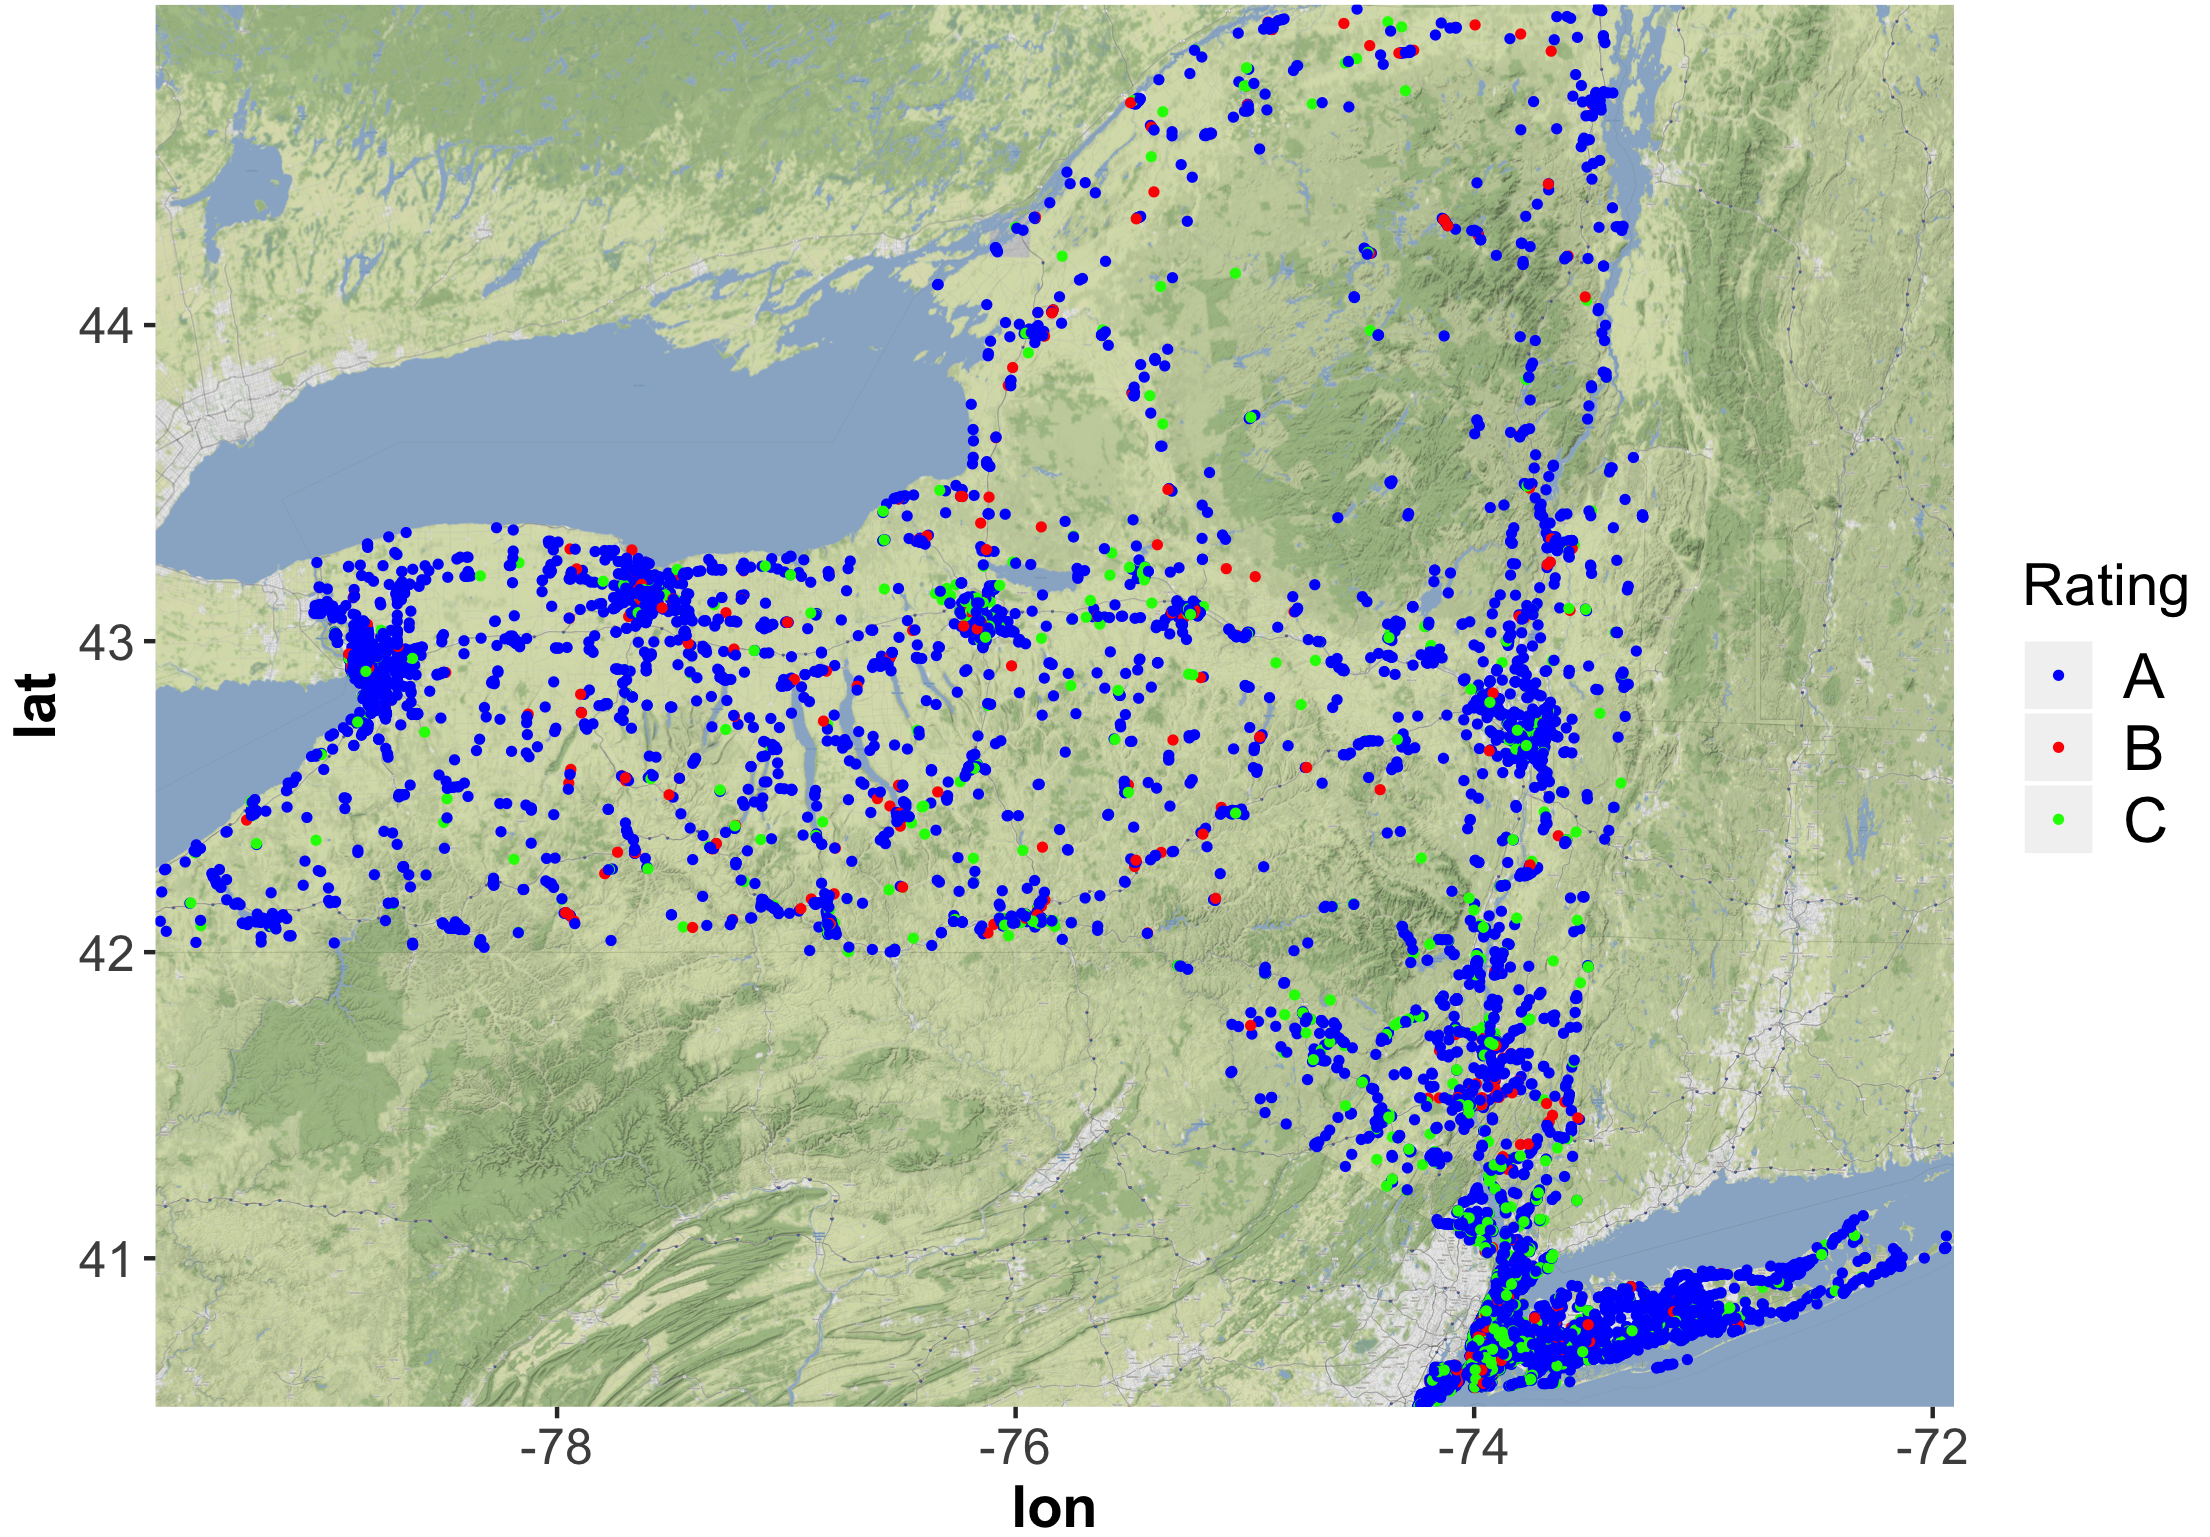
\includegraphics[width=0.5\textwidth]{Plots/Plot1_Map.png}
     }
     \hfill
     \subfloat[New York City]{%
       \includegraphics[width=0.5\textwidth]{Plots/Plot2_Map.png}
     }
\end{figure}
With complete spatial information, we now compute the two variables "shops density in 1km radius" as well as "rating of the closest neighbor". The distances of coordinates in meters are calculated with the Haversine Formula\footnote{The Haversine Formula has its roots in spherical trigonometry and calculates the geodesic distance -- the shortest path between two points on a curved surface of a sphere, like the earth. It needs to be mentioned that Haversine Formula does not take into account changes in altitude \citep[pp. 157 - 160]{haversine}. However, it provides sufficient accuracy for the scope of this project.}
\begin{align*}d = R \left( 2 \atantwo (\sqrt{a}, \sqrt{1-a} )  \right) \qquad a = \sin^{2}(\frac{\Delta\alpha}{2}) + \cos(\alpha_{1})\cos(\alpha_{2})\sin^{2}(\frac{\Delta\lambda}{2}) \end{align*}
where $\alpha_{i}$ are latitudes, $\lambda_{i}$ are longitudes and $R$ is the earth's radius ($6371\times10^{3}m$).

\subsection{Subway Data}

We amend the New York City inspection data with location information of subway stations. We use again \href{https://data.ny.gov/Transportation/NYC-Transit-Subway-Entrance-And-Exit-Data/i9wp-a4ja}{an official dataset provided by the State of New York}. The dataset contains the location of every subway station. We apply again the Haversine Formula to find the distance of the closest station to every shop.

\subsection{Google Web Scraper}

While doing research to find datasets with regards to food inspections we decided to obtain more information from webpages. The reviews from customers, written on google places, could give us information about how individual persons perceived their visit to the specific food shop. In order to gather this information from the internet we set up a web scraper. We used the package \textit{RSelenium} to execute an automated google search for all the observations. This included a lot of trial and error due to unforeseen changes of the xPaths and other errors. Most of the errors only showed up in the middle of the scraping process, which had a duration of about 24 hours for all the food shops. Therefore, it was only possible to adjust the function after the script run during the night. This resulted in a lot of waiting and adjusting but finally the data was scraped successfully.\\

A brief analysis of the dataset revealed the incompleteness of the ratings. Approximately 40\% of the shops don't have an entry in google places and thus no rating. After a lot of discussion on how to handle the problem we agreed on using the number of reviews as a parameter of the internet popularity and assign all the missing shop a value of $0$. 

\subsection{Airbnb Data}

In order to acquire additional data on the location of the shops, we integrated data from Airbnb (average price and number of rooms). To join the original and the airbnb data frames, a matching key is needed. We use latitude and longitude to assign every Airbnb observation to a ZIP code. Thereafter, we grouped the data by ZIP code, calculated the respective means and counts and added it to the new tibble.

\section{Data Analysis}

\subsection{The Class Imbalance Problem}\label{Imbalance Problem}
Closer scrutiny of Figure~\ref{map1} sheds light on the extremely imbalanced distribution of the original data. In fact, the rating A contributes to XX\% on state level while B and C are only represented to XX\% and XX\% respectively. This differences in the occurrence has a large impact on the prediction capabilities of a model. The univariate linear discriminant analysis (LDA) illustrates the issue. The LDA decision rule is
\begin{equation*}\delta_{k}(x) = x \frac{\mu_{k}}{\sigma^{2}} - \frac{\mu_{k}^{2}}{2\sigma^{2}} + log(\pi_{k})\end{equation*}
with the decision boundary for two classes equal to
\begin{equation*}\delta_{1}(x) = \delta_{2}(x) \Leftrightarrow x = \frac{\mu_{1} + \mu_{2}}{2} + log\left(\frac{\pi_2}{\pi_{1}}\right)\frac{\sigma^{2}}{\mu_{1} - \mu_{2}}.\end{equation*}
If the two classes are perfectly equally represented, the prior probabilities are $\pi_{1} = \pi_{2}$ and the $\log$ term gets zero. In the presence of highly skewed classes, in turn, $\pi_{1}$ and $\pi_{2}$ are different from each other. If class 1 occurs more often it holds that $\lim_{x \to 0^{+}}log(x) = -\infty \Leftrightarrow \lim_{\pi_{1} \to 1 (\pi_{2} \to 0^{+})}log(\frac{\pi_{2}}{\pi_{1}}) = -\infty$. So, the following three extreme cases for decision boundaries can be distinguished:
\begin{align*} x = \lim_{\pi_{1} \to 1} \frac{\mu_{1} + \mu_{2}}{2} -\infty \qquad  x = \frac{\mu_{1} + \mu_{2}}{2} \text{ with } \pi_1 = \pi_2 \qquad x = \lim_{\pi_{1} \to 0^{+}} \frac{\mu_{1} + \mu_{2}}{2} -\infty \end{align*}
Hence, an imbalance of the two classes moves the decision boundary infinitely to the right or to the left respectively. As a consequence, the model will always predict the class that is heavily overrepresented and ignore the others. The methodology presented in the next chapter will exactly address this issue and improve the prediction accuracy of inspection grades B and C.

\subsection{Analysis Methodology}

\citet[p. ]{James} use bagging to reduce the variance in tree models. However, instead of taking a random subset of the entire data like in normal bagging, we use repeated subsets that show an equal distribution of the three classes. Therefore, we either take more observations from the B or C classes (oversampling) or we remove a part of the observations from the A class (undersampling). \citet[p. 83]{imbalance} outlines that both approaches have drawbacks. While oversampling increases the likelihood for overfitting since we create exact copies of a minority class, undersampling ignores potentially useful data points. To address these weaknesses, we combine over- and undersampling with bagging which results in over- and under-bagging. We combine this approach with a forward-stepwise-selection that is suggested by \citet[p. ]{James}. In detail, we apply the following procedure:
\begin{enumerate}
\item Take a subset of the data where the three classes are balanced either with over- or undersampling
\item Use K-Fold Cross-Validation (CV) to get cross-validated errors from this subset
\item Repeat the entire process B times and then take the average rate of the CV-errors to get the bagged-CV-errors
\end{enumerate}
After we found the model with the lowest bagged-CV-error, we estimate the model B times and then we take majority vote of all the B models to classify the observation to one of the three categories.

\subsection{Pre-Analysis Variable Elimination}
The obvious drawback of the described methodology is that it is computationally intensive. Using all XX variables would be accordingly difficult given the extent of this project. A boosting model with 100 variables, for instance, would run for XX hours. Furthermore, some of the demographic variables are anyways linear combinations of each other and must be excluded from our analysis. For the remaining ones, we calculate the correlation to the Inspection Grade we want to predict and take the 20 covariates with the highest correlation.



\section{Conclusion}
--> Wrong predictors


\newpage

\bibliographystyle{apacite}
\bibliography{bibliography}

\end{document}